% kuleuventheme2 by Janez Kren, September 2017, janez.kren@kuleuven.be, based on:
% kuleuventheme 1.3 by Roland Pastorino, 2013 roland.pastorino@kuleuven.be / www.rolandpastorino.com

\PassOptionsToPackage{usenames, table, dvipsnames}{xcolor} % 
\documentclass[11pt,t]{beamer}
\usetheme{kuleuven2}	%THEME OPTIONS for LOGO: kul (default), kulak, lrd,    ; OPTIONS for TITLE PAGE: normal (default), sedes


%%% OTHER SETTINGS
\usefonttheme[onlymath]{serif}			% math font with serifs, delete to make it sans-serif
\setbeamertemplate{footline}[body] 		% delete this line to remove footline bar on all frames
%\usepackage[orientation=landscape,size=custom,width=16,height=9,scale=0.5,debug]{beamerposter} %enable for widescreen 16:9 ratio
%\titlegraphic{ \includegraphics[width=.2\paperwidth]{mytitlepagepic.png} } %optional title page image


%%% ADDED BY ALEX (start)
\usepackage[english]{babel}
\usepackage{amsfonts}
\usepackage{amssymb}

\usepackage{pythonhighlight}

\usepackage[orientation=landscape,size=custom, width=16,height=9,scale=0.5,debug]{beamerposter} 

\definecolor{mygray}{rgb}{0.8,0.8,0.8}
\newcommand{\inline}[1]{ \colorbox{mygray}{\lstinline{#1}}}

\usepackage{xcolor}

\usepackage{layouts} % To get text/page width

\usepackage{listings}
\definecolor{codegreen}{rgb}{0,0.6,0}
\definecolor{codegray}{rgb}{0.5,0.5,0.5}
\definecolor{codepurple}{rgb}{0.58,0,0.82}
% \definecolor{backcolour}{rgb}{0.95,0.95,0.92}
\definecolor{backcolour}{rgb}{0.93,0.93,0.95}
\lstdefinestyle{mystyle}{
    backgroundcolor=\color{backcolour},   
    commentstyle=\color{codegreen},
    keywordstyle=\color{magenta},
    numberstyle=\tiny\color{codegray},
    stringstyle=\color{codepurple},
    basicstyle=\ttfamily\footnotesize,
    breakatwhitespace=false,         
    breaklines=true,                 
    captionpos=b,                    
    keepspaces=true,                 
    numbers=left,                    
    numbersep=5pt,                  
    showspaces=false,                
    showstringspaces=false,
    showtabs=false,                  
    tabsize=2
}
\lstset{style=mystyle}

%%% ADDED BY ALEX (stop)


%%% TITLE PAGE INFO:
\title[Geavanceerde Computerarchitectuur 2$^{\text{nd}}$ session]{Geavanceerde Computerarchitectuur 2$^{\text{nd}}$ session} %[]] will appear in footline
\subtitle{Race conditions}

\author{Thomas Feys, {\footnotesize thomas.feys@kueluven.be}}
\institute{DRAMCO -- WaveCore -- ESAT}
\date{}




\begin{document}
\csname beamer@calculateheadfoot\endcsname %recalculate head and foot dimension


 %%
 %%  0. TITLE PAGE and TABLE OF CONTENT
 %%
% Title page
\begin{frame}[plain,noframenumbering]
	\titlepage
\end{frame}
	

% Table of Contents
\begin{frame}{Outline}
	\hfill	{\large \parbox{.961\textwidth}{\tableofcontents[hideothersubsections]}}
\end{frame}







\section{Race conditions}


\begin{frame}{Race conditions} 
    \vspace{-2mm}
    \begin{figure}
        \centering
        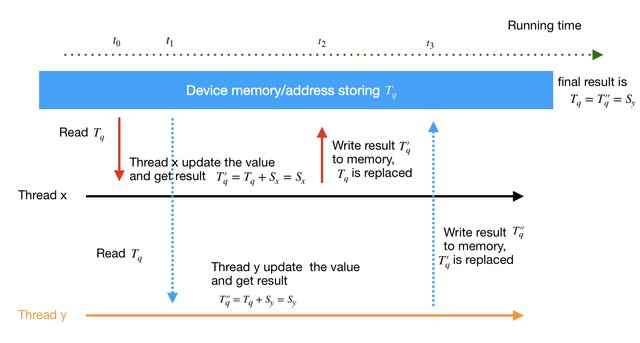
\includegraphics[width=0.84\linewidth]{figure/session-2/race.jpg}
    \end{figure}
\end{frame}


\begin{frame}{Addition - an example of possible race conditions}
    \vspace{5mm}
    \begin{figure}
        \centering
        

\begin{tikzpicture}[]



%%% DRAWING %%%%%%%%%%%%%%%%%%%%%%%%%%%%%%%%%%%%%%%%%%%%%%%%%%%%%%%%%%%%%%%%%



\foreach \x in {0,...,7} {

    \draw[black] (\x, 0) rectangle ++ (1, 1);
    
    \draw[black] (\x, -3) rectangle ++ (1, 1);
   
    \node[anchor=center, align=center] at (\x+0.5, 0.5) {\x};
    
    \node[anchor=center, align=center] at (\x+0.5, -0.25) {$+\!\!=$};

    \draw[-{angle 60}] (\x+0.5, -0.5) to[out=-90, in=90] (0.5,-2);
    
    \node[anchor=center, align=center] at (\x+0.5, -2.5) {\x};
    
}

\fill[white] (0.1, -2.9) rectangle ++ (0.8, 0.8);
\node[anchor=center, align=center] at (0.5, -2.5) {\textbf{?}};


\draw[gray] (0.5, -2.5) circle (1cm);
\node[gray, anchor=center, align=center] at (0.5, -3.75) {Result};


\end{tikzpicture}
    \end{figure}
\end{frame}


\begin{frame}{Resource locking and waiting as an alternative}
    \vspace{-2mm} 
    \begin{figure}
        \centering
        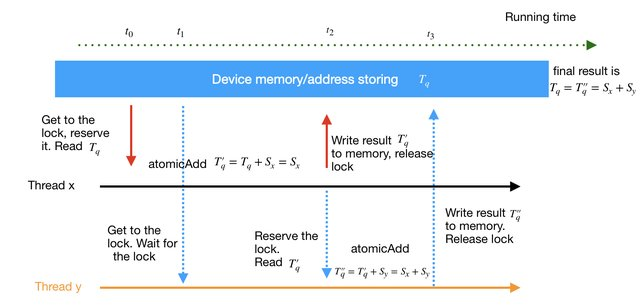
\includegraphics[width=0.90\linewidth]{figure/session-2/atomic.jpg}
    \end{figure}
\end{frame}


\begin{frame}{Atomic operation} 

    An atomic command gets executed without interruption
    
    \vspace{2mm}
    
    Threads get \textbf{sequential access} to a common resource
    
    \vspace{6mm}
    
    \uncover<2->{
    CUDA (and other interfaces) features built-in atomic functions:
    
    \vspace{2mm}
    
    \begin{itemize}\setlength\itemsep{0.5em}
        \item For addition \inline{atomicAdd(...)}
        \item For subtraction \inline{atomicSub(...)}
        \item For minimum detection \inline{atomicMin(...)}
        \item For maximum detection \inline{atomicMax(...)}
        \item ... full list and reference on p. 187--190 of the programming guide
    \end{itemize}
    }

\end{frame}


\begin{frame}{Semi-parallel addition using reduction} 

    \begin{columns}[t]
    \begin{column}{.5\textwidth}
        \begin{figure}
            \centering
            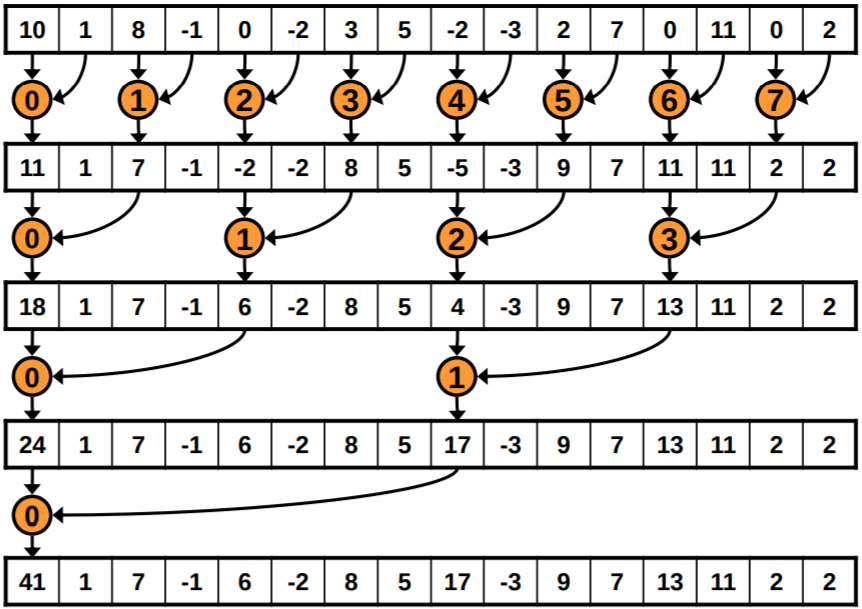
\includegraphics[width=0.9\columnwidth]{figure/session-2/reduction.png}
        \end{figure}
    \end{column}
    \begin{column}{.52\textwidth}
    {\small
    \begin{itemize}\setlength\itemsep{1em}
        \uncover<2->{\item Ideal for $2^N$ long inputs}
        \uncover<3->{\item Complexity $\mathcal{O}(\log_2(N))$}
        \uncover<4->{\item Synchronize threads on each reduction step to avoid race conditions (see p. 173)}
        \uncover<5->{\item Shifting direction not important}
    \end{itemize}
    }
    \end{column}
    \end{columns}

\end{frame}


\section{Exercise}

\begin{frame}{Max detection using three approaches} 

    Implement max detection using:
    \vspace{1mm}
    \begin{itemize}\setlength\itemsep{0.75em}
        \item A for loop on the CPU,
        \item A GPU kernel employing atomic operation, and
        \item A GPU kernel using reduction.
    \end{itemize}
    
    \vspace{3mm}
    
    Use a 1D input array of your liking.
    
    \vspace{3mm}
    
    Assess the dependency of the execution time on the input array's length.
    
    \vspace{3mm}

    \textit{Timing examples are provided in the cheat sheet.}

\end{frame}

\begin{frame}{Tips}
Start simple, only consider 1 block!

\vspace{2mm}

Many ways to accomplish the same goal

\vspace{2mm}

Some ways might use shared memory (more in lab 4)

\begin{itemize}\setlength\itemsep{1em}
    \item Memory is shared per block (all threads in block can access it)
    \item \inline{extern __shared__ int sdata[];}
    \item Calling a kernel with shared memory \inline{foo<<<nr_blocks, nr_threads, size_shared_memory>>>}
\end{itemize}

\end{frame}


\begin{frame}{Guiding questions} 

    \begin{itemize}\setlength\itemsep{1em}
        \item \textbf{Is the result correct?}
        \item \textbf{How does time increase as a function of input size?}
        \item What happens if the input is larger than 2048 (how would you ensure correct calculation and are there additional synchronization steps)?
        \item Consider calling the kernel with much less threads than there are data elements. For example, one tenth. How would you ensure all elements get processed?
        \item How would you tackle a 2D array?
    \end{itemize}

\end{frame}

\end{document}
